% 
% Annual Cognitive Science Conference
% Sample LaTeX Paper -- Proceedings Format
% 

% Original : Ashwin Ram (ashwin@cc.gatech.edu)       04/01/1994
% Modified : Johanna Moore (jmoore@cs.pitt.edu)      03/17/1995
% Modified : David Noelle (noelle@ucsd.edu)          03/15/1996
% Modified : Pat Langley (langley@cs.stanford.edu)   01/26/1997
% Latex2e corrections by Ramin Charles Nakisa        01/28/1997 
% Modified : Tina Eliassi-Rad (eliassi@cs.wisc.edu)  01/31/1998
% Modified : Trisha Yannuzzi (trisha@ircs.upenn.edu) 12/28/1999 (in process)
% Modified : Mary Ellen Foster (M.E.Foster@ed.ac.uk) 12/11/2000
% Modified : Ken Forbus                              01/23/2004
% Modified : Eli M. Silk (esilk@pitt.edu)            05/24/2005
% Modified : Niels Taatgen (taatgen@cmu.edu)         10/24/2006
% Modified : David Noelle (dnoelle@ucmerced.edu)     11/19/2014

%% Change "letterpaper" in the following line to "a4paper" if you must.

%%% MAX = 6 Pages (including references)

\documentclass[10pt,letterpaper]{article}

\usepackage{cogsci}
\usepackage{pslatex}
\usepackage{graphicx}
\usepackage{apacite}
\usepackage{color}


\title{Word identification under multimodal Uncertainty}
 
\author{{\large \bf Abdellah Fourtassi} \\ afourtas@stanford.edu \\
  Department of Psychology\\ Stanford University\\
  \And {\large \bf Michael C. Frank}\\ mcfrank@stanford.edu \\
  Department of Psychology\\ Stanford University}


\begin{document}

\maketitle


\begin{abstract}

Language requires the ability to process arbitrary multimodal input. It also requires the ability to infer categories under uncertainty. In this paper, we introduce a task that allows us to examine how adults identify word categories under uncertainty from the auditory and the visual modality. We propose a Bayesian model of the task which provides an optimal baseline. The predictions are tested in two experiments where category recognition is made under two kinds of uncertainty: ambiguity and noise. In both cases, human data shows many patterns of optimal behaviour, and the baseline explains most of the variance. However, when one modality is noisy, we found evidence for a systematic preference for the non-noisy modality.

\textbf{Keywords:} 
Language; audio-visual processing; word learning; speech perception; computational modeling. 
\end{abstract}

Language uses symbols expressed in one modality (e.g., the auditory modality in the case of speech) to communicate about things in the world, which we perceive through  various sensory modalities (e.g., the visual modality in the case of concrete objects). Therefore, understanding language requires the ability to process arbitrary multisensory input. This processing, however, is only a first step. When a speaker utters a word and points to an object, it is not enough for the observer to be able to encode these precise sound and object tokens. They should, on top of that, be able to identify the underlying categories (such as the phonemes, the concept, and the word category). This challenge is quite obvious when a person has to learn these categories (e.g., a baby who starts learning language). But a challenge is present even when the person already knows the categories, but has to recognize them. This is because individual tokens are often ambiguous or/and noisy\cite<e.g.,>{hillenbrand1995}. They do not indicate with absolute certainty their category membership, they do so only in probabilistic terms. For example, the speaker may make a mispronunciation, or their utterance may get distorted because of ambient noise. Similarly, the identity of the object that is being referred to may be uncertain when there exist other surrounding and/or similar looking objects, or when the observer's view is partially obstructed.

It follows that, in order to identify the speaker's intended categories, an observer has to be able to reason under a great deal of uncertainty. To characterize this ability, it has been suggested that people encode tokens with their probability distributions, base their decisions on these probabilities, and adjust their behavior when these probabilities change \cite<e.g.,>{clayard08}. However, previous work in this line of research has largely focused on the unimodal case, that is, when categories can be defined along one modality, such as the phonemes \cite<e.g.,>{feldman2009}. A few studies did explore some aspects of cross-modal processing in this framework \cite<e.g.,>{bejjanki2011, kleinschmidt2015}, but focused on the specific case of phoneme recognition from speech and lip movement, wherein people assume information from both modalities to be tightly correlated. 

In the present work, we study the case of word category recognition, where a word is an \textit{arbitrary} mapping between a sound category and a visual category. We test people on their ability to encode audio-visual tokens and use them to recognize the underlying word category. Crucially, this recognition is made under uncertainty from both the auditory category (the phoneme) and the visual category (the concept being referred to). Our goal is to explore how adults deal with such multimodal ambiguity in a categorical task. To this end, we propose a model that combines uncertainty in an optimal way, and we use it as a baseline for human data. More precisely, we examine the extent to which human data conform to, or deviate from the baseline, and whether the deviation involves a systematic preference for a particular modality?

The paper is organized as follows. First, we introduce our audio-visual word recognition task. Second, we present the model and explain how it generate an optimal baseline. Then we present the behavioral experiments where we test category recognition under audio-visual uncertainty. In experiment 1, audio-visual tokens are clear but their category membership is ambiguous.  In experiment 2, input to one modality is ambiguous, and input to the other is ambiguous as well as noisy. We analyse and discuss the results of the experiments in the light of the model's predictions.

\section{The audio-visual word recognition task}

We introduce a new task that tests audio-visual category recognition. We use two visual categories (cat and dog) and two auditory categories (/b/ and /d/ embedded in the minimal pair /aba/-/ada/). For each participant, an arbitrary pairing is set between the auditory and the visual categories, leading to two audio-visual word categories (e.g., dog-/aba/, cat-/ada/). 

In each trial, participants are presented with an audio-visual target (the prototype of the target category), immediately followed by an audio-visual test. 
The test may differ from the target in both the auditory and the visual components. The auditory component is sampled from a continuum along the second formant (F2) linking the words /aba/ and /ada/. The visual component is sampled from a morph that links the prototypical pictures of the dog and the cat.  After these two presentations, participants are instructed to press `same' or `different'. 

This task is similar to the task introduced by \citeA{sloutsky2003} and used in subsequent research to probe audio-visual encoding. However, unlike this previous line of research, here participants are not asked whether the two audio-visual presentations are identical, instead, they are asked to press `same' if they think the second item (the test) belonged to the same word category as the prototype (e.g.,  dog-/aba/), even if there is a slight sound mispronunciation,  a slight difference in the object’s shape, or a slight difference in both the pronunciation and the shape. They are instructed to press `different' if they think that the test was, rather, an audio-visual instance to the other word category (cat-/ada/).

As shown in figure \ref{fig:task}, besides the audio-visual trials where both the sounds and the pictures are presented, there are also unimodal trials where the pictures are hidden (auditory-only) or where the sounds are muted (visual-only). These unimodal trials are crucial since they provide us with the probability distributions of the auditory and visual categories over their tokens. In fact, the goal is to examine whether participants' responses on the bimodal trial are optimal combination of the probabilities derived from their responses on the unimodal trials. 

Next, we explain how we modeled this task in a Bayesian framework. 

\begin{figure}[tp]
\centering
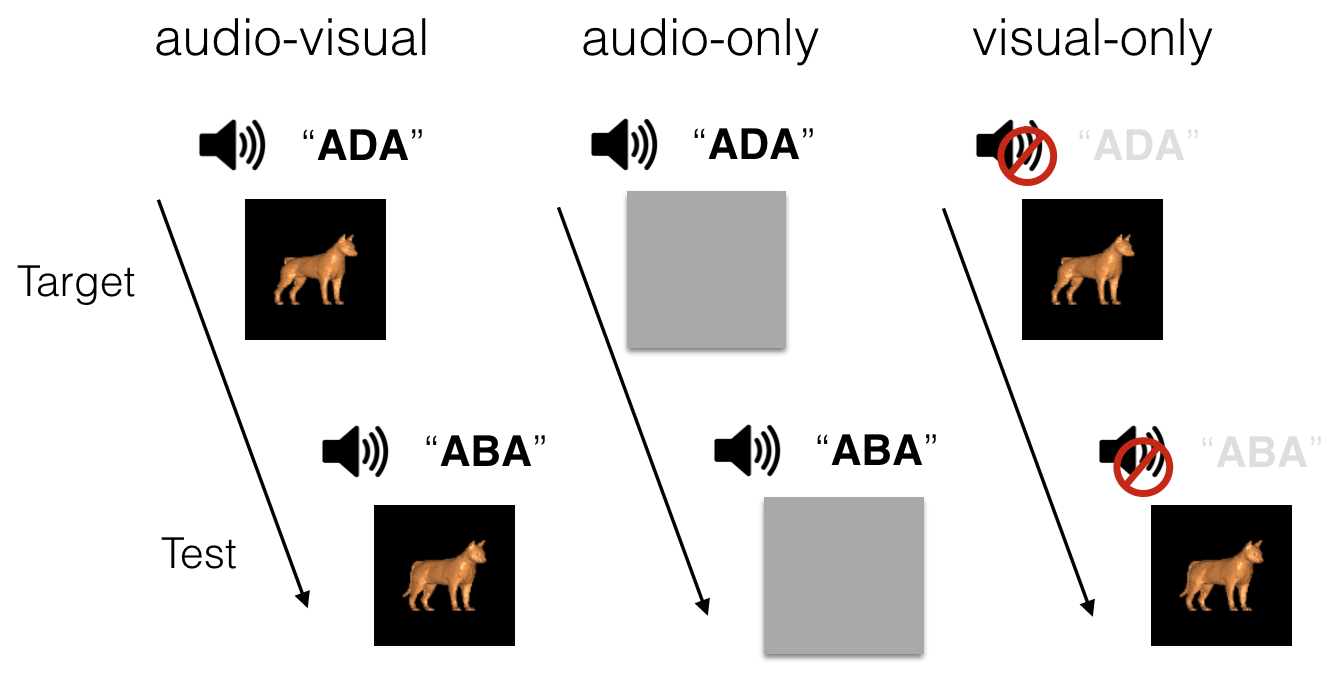
\includegraphics[width=0.4\textwidth]{task1.png}
\caption{Overview of the task}
\label{fig:task}
\end{figure}

\section{What would an ideal recognizer do?}
 
The unimodal conditions (auditory-only or visual-only)  are used to characterize the probability distributions of the auditory and the visual categories.  We assume, for the sake of simplicity, that the probability distributions are normally distributed:

$$ a | A \sim  N(\mu_A, \sigma^2_A) $$
$$ v | V \sim  N(\mu_V, \sigma^2_V) $$

In each modality, we have two categories: /ada/ ($A=1$) and /aba/ ($A=2$) in the auditory dimension, and \textit{cat} ($V=1$) and \textit{dog} ($V=2$) in the visual dimension (the identity of the categories was randomized in the experimental setup).

In the bimodal condition, participants see word tokens made of audio-visual input, and have to make a categorical decision. We represent word tokens as vectors in the audio-visual space $\mathbf{w}=(a,v)$.
A word category $W$ is defined as the joint distribution of the auditory and visual categories. It can be characterized with a bivariate normal distribution in the audio-visual space:
$$ \mathbf{w} | W \sim  N(M_W, \Sigma_W) $$
\begin{figure}[tp]
\centering
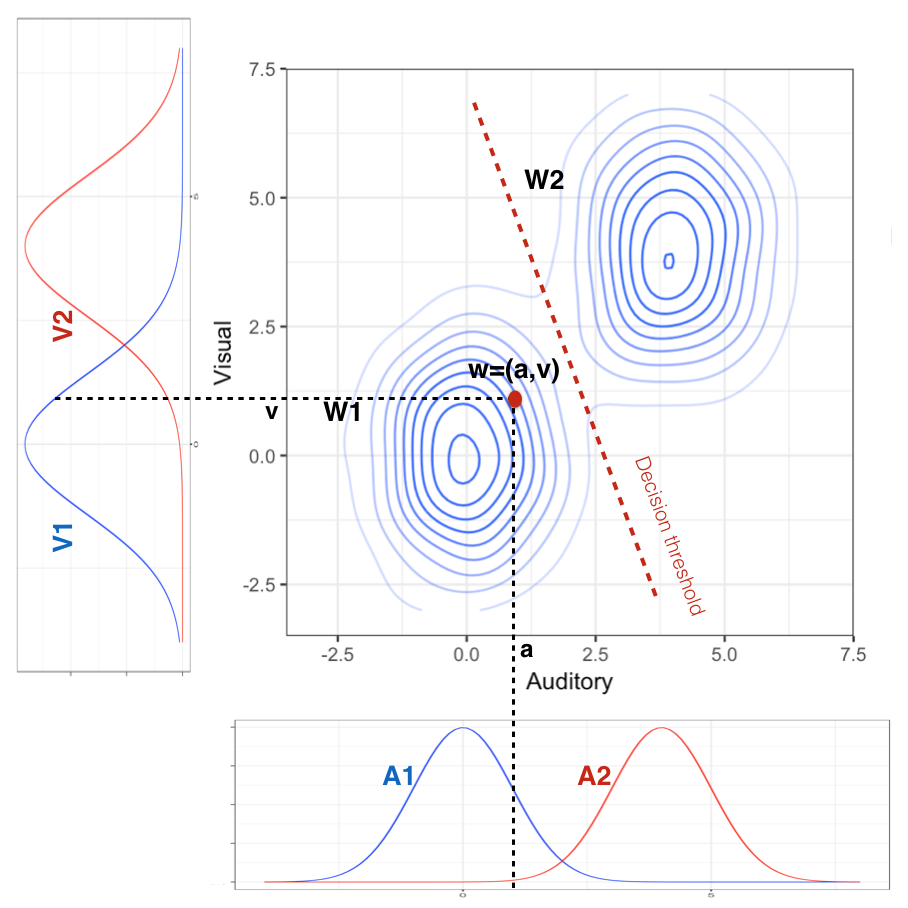
\includegraphics[width=0.4\textwidth]{MyTask.png}
\caption{Model of the task: a word category is defined as the joint bivariate distribution of an auditory category (bottom) and a visual semantic category (left). Upon the presentation of a word token $w$, participants guess whether it is sampled from the word category $W1$ or from $W2$. Decision threshold is where the guess probability is 0.5. (Plotted distributions are for illustration only)}
\label{fig:space}
\end{figure}
We have two word categories: dog-/aba/ ($W=1$) and cat-/ada/ ($W=2$). Participants can be understood as choosing one of these two word categories (figure \ref{fig:space}). For an ideal ``recognizer'', the probability of choosing category 2 when presented with an audio-visual instance $\mathbf{w}=(a,v)$ is the posterior probability of this category:
\begin{equation}
\small
p(W=2 | \mathbf{w})=\frac{p(\mathbf{w}|W=2)p(W=2)}{p(\mathbf{w}|W=2)p(W=2)+p(\mathbf{w}|W=1)p(W=1)}
\end{equation}
We make the assumption that, given a particular word category, the auditory and visual tokens are independently generated:
\begin{equation}
p(\mathbf{w} | W) = p(a,v| W) = p(a| W)p(v| W)
\end{equation}

Under this assumption, the posterior probability reduces to:
\begin{equation}
p(W=2 | \mathbf{w})=\frac{1}{1+(1+\epsilon)\exp(\beta_0+\beta_aa+\beta_vv)}
\label{eq:pred}
\end{equation}

with $\beta_a=\frac{\mu_{A1}-\mu_{A2}}{\sigma^2_{A}}$, 
$\beta_v=\frac{\mu_{V1}-\mu_{V2}}{\sigma^2_{V}}$,
$\beta_0=\frac{\mu^2_{A2}-\mu^2_{A1}}{2\sigma^2_{A}}+\frac{\mu^2_{V2}-\mu^2_{V1}}{2\sigma^2_{V}}$

and $1+\epsilon=\frac{p(W=1)}{p(W=2)}$ is the proportion of the prior probabilities. If the identity of word categories is randomized, and if $W1$ is the target, then $\epsilon$ measures a response bias to `same' if $\epsilon > 0 $, and a response bias to `different' if $\epsilon < 0 $.

In sum, the posterior \ref{eq:pred} provides a baseline for how probabilities that characterize uncertainty in each modality can be combined to make categorical decision about bimodal input.

Next, we present the behavioral experiments. Our goal is twofold: 1) examine the extent to which human responses correspond or deviate from the predictions of the optimal baseline. 2) if there is a deviation from the baseline, examine whether this deviation involves a systematic preference for a particular modality.

\section{experiments}

In experiment 1, we test the predictions of the model in the case where uncertainty is due to ambiguity in terms of category membership. 

\subsection{experiment 1}

\subsubsection{Participants}
We planned to run 100 participants recruited from Amazon Mechanical Turk. Only participants with US IP addresses and a task approval rate above 85\% were allowed to participate. They were paid at an hourly rate of \$6/hour.  Data
were excluded if participants completed the task more than
once (2 participants). Moreover, as specified in the preregistration (\url{https://osf.io/h7mzp/}), participants were excluded if they had less than 50\% accurate responses on the unambiguous training trials (6), and if they reported having experienced a technical problem of any sort during the online experiment (14). The final sample consisted of 76 participants.

\subsubsection{Stimuli}
For the auditory stimuli, we used the continuum introduced in \citeA{vroomen2004}. It is a 9-point /aba/--/ada/ speech continuum which was created by varying the frequency of the second (F2) formant in equal steps. We selected 5 equally spaced points from the original continuum by keeping the end-points (prototypes) 1 and 9, as well as the three points: 3, 5, and 7 along the continuum.

For the visual stimuli, we used a morph continuum introduced in \citeA{freedman2001}. In the original stimuli, a continuous set of images was generated from three cat prototypes and
three dog prototypes. We selected a morph along the dog and cat prototypes that seemed most natural. Moreover, from the original 14 points, we selected 5 points as follows: we kept the item that seemed most ambiguous (point 8), the 2 preceding points (i.e., 7 and 6) and the 2 following points (i.e., 8 and 9). The 6 and 9 points along the morph were quite distinguishable, and we took them to be our prototypes (figure \ref{fig:morph}).

\begin{figure}[tp]
\centering
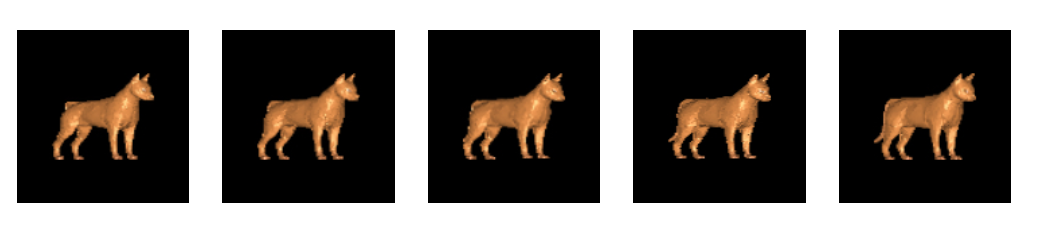
\includegraphics[width=0.4\textwidth]{morph.png}
\caption{Visual stimuli}
\label{fig:morph}
\end{figure}


\subsubsection{Design and Procedure}
We told participants that an alien was naming two objects: a dog, called /aba/ in the alien language, and a cat called /ada/. In each trial, we presented the first object (the target) on the left side of the screen simultaneously with the corresponding sound. The target was always the same (e.g., dog-/aba/). The second sound-object pair (the test) followed after half a second. It showed up on the right side of the screen and was supposed to be either another dog-/aba/, or a cat-/ada/. For both the target and the test, we displayed the object when the corresponding sound started playing, and we made it disappear when the sound stoped (for a total of around 800ms). For each participant, we randomized the sound-object mapping as well as the identity of the target. Finally, we instructed participants to press S (for same) if they thought the alien was naming another dog-/aba/, and D (for different) if they thought the alien was naming a cat-/ada/. 


The first part of the experiment was a training to familiarize the participants with the task and the stimuli. In this training phase, we used only the prototype pictures and the prototype sounds, and each trial had a correct answer: the test item was either exactly the same as the target, or the prototype of the other word category. There were a total of 12 trials, half same, and half different. The second part was the real task. In this part, we told participants that, like in the training, the first sound-object pair would be the same. However, in the second pair, both the sound and the picture could be ambiguous. We told them that each trial was different. Finally, we encouraged participants to base their answers on both the sounds and the pictures in the bimodal condition. Each test item was made of a sound sampled from the /aba/-/ada/ continuum, and the picture form the dog-cat morph. There was a total of 25 possible combinations in the bimodal condition, and 5 in each of the unimodal conditions. Each participants answered twice to each possible trial in each condition for a total of 70 trials/participants. For each participant,  we randomized the order of conditions (auditory-only, visual-only, and bimodal). We designed the experiment to take between 10 to 15 minutes to complete.
\begin{figure}
\centering
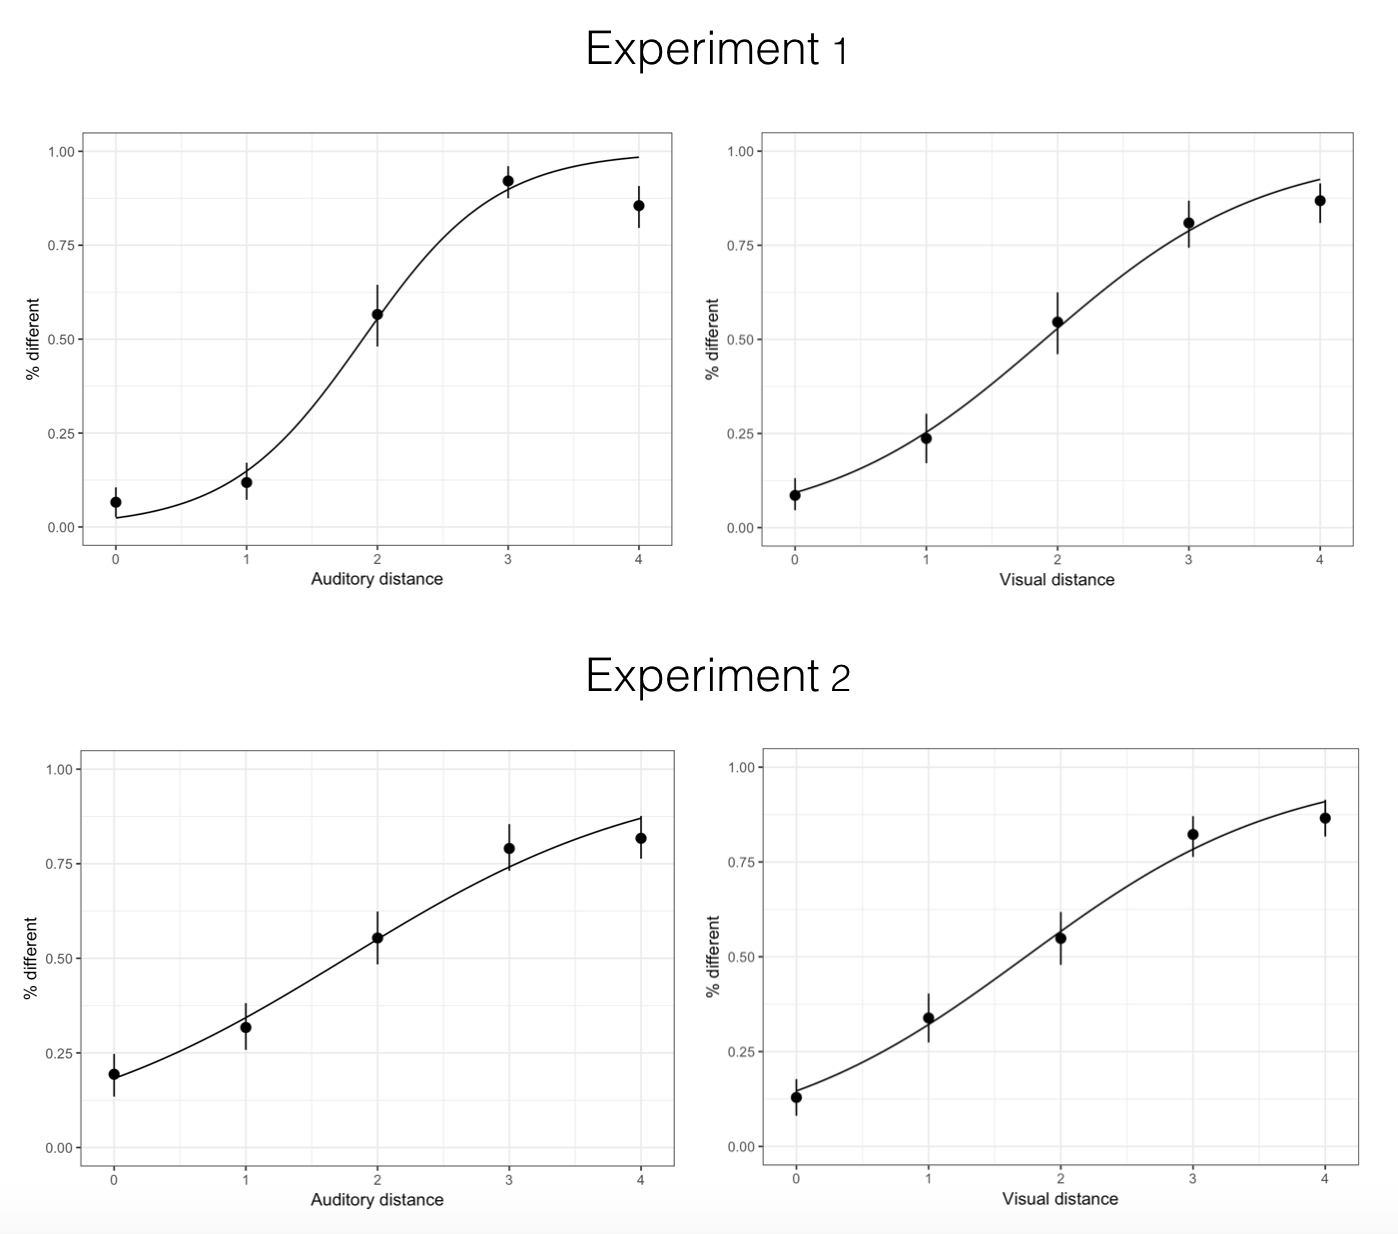
\includegraphics[width=0.4\textwidth]{unimodal.png}
\caption{Average human responses in the auditory-only condition (left), and visual-only condition (right). Error bars are 95\% confidence intervals. Solid lines represent the unimodal fits. }
\label{fig:unimodal}
\end{figure}


\subsubsection{Results}

\begin{figure}[h]
\centering
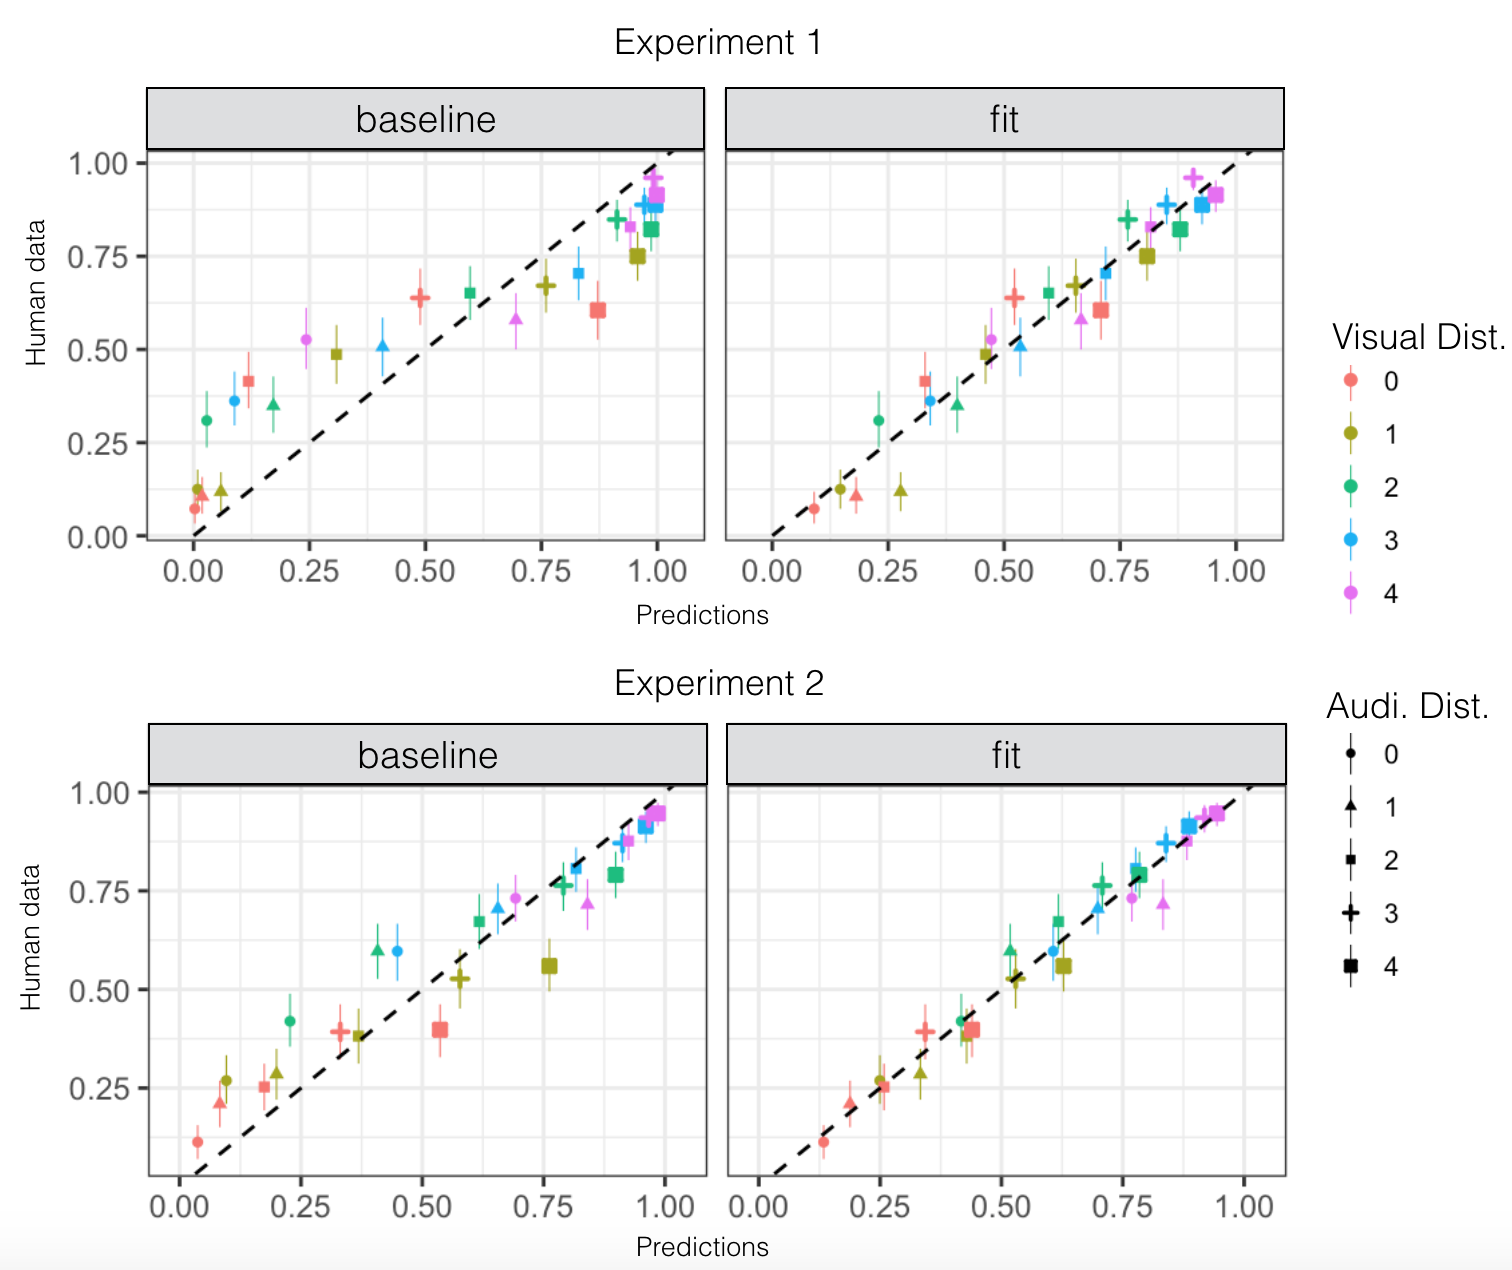
\includegraphics[width=0.4\textwidth]{correlation.png}
\caption{Human responses vs. the baseline predictions. Error bars are 95\% confidence intervals. In experiment 1, the baseline and the fit explained 89\%, and 94\% of total variance, respectively. In experiment 2, the baseline and the fit explained 91\%, and 97\% of total variance, respectively}
\label{fig:corr}
\end{figure}

\begin{figure*}
\centering
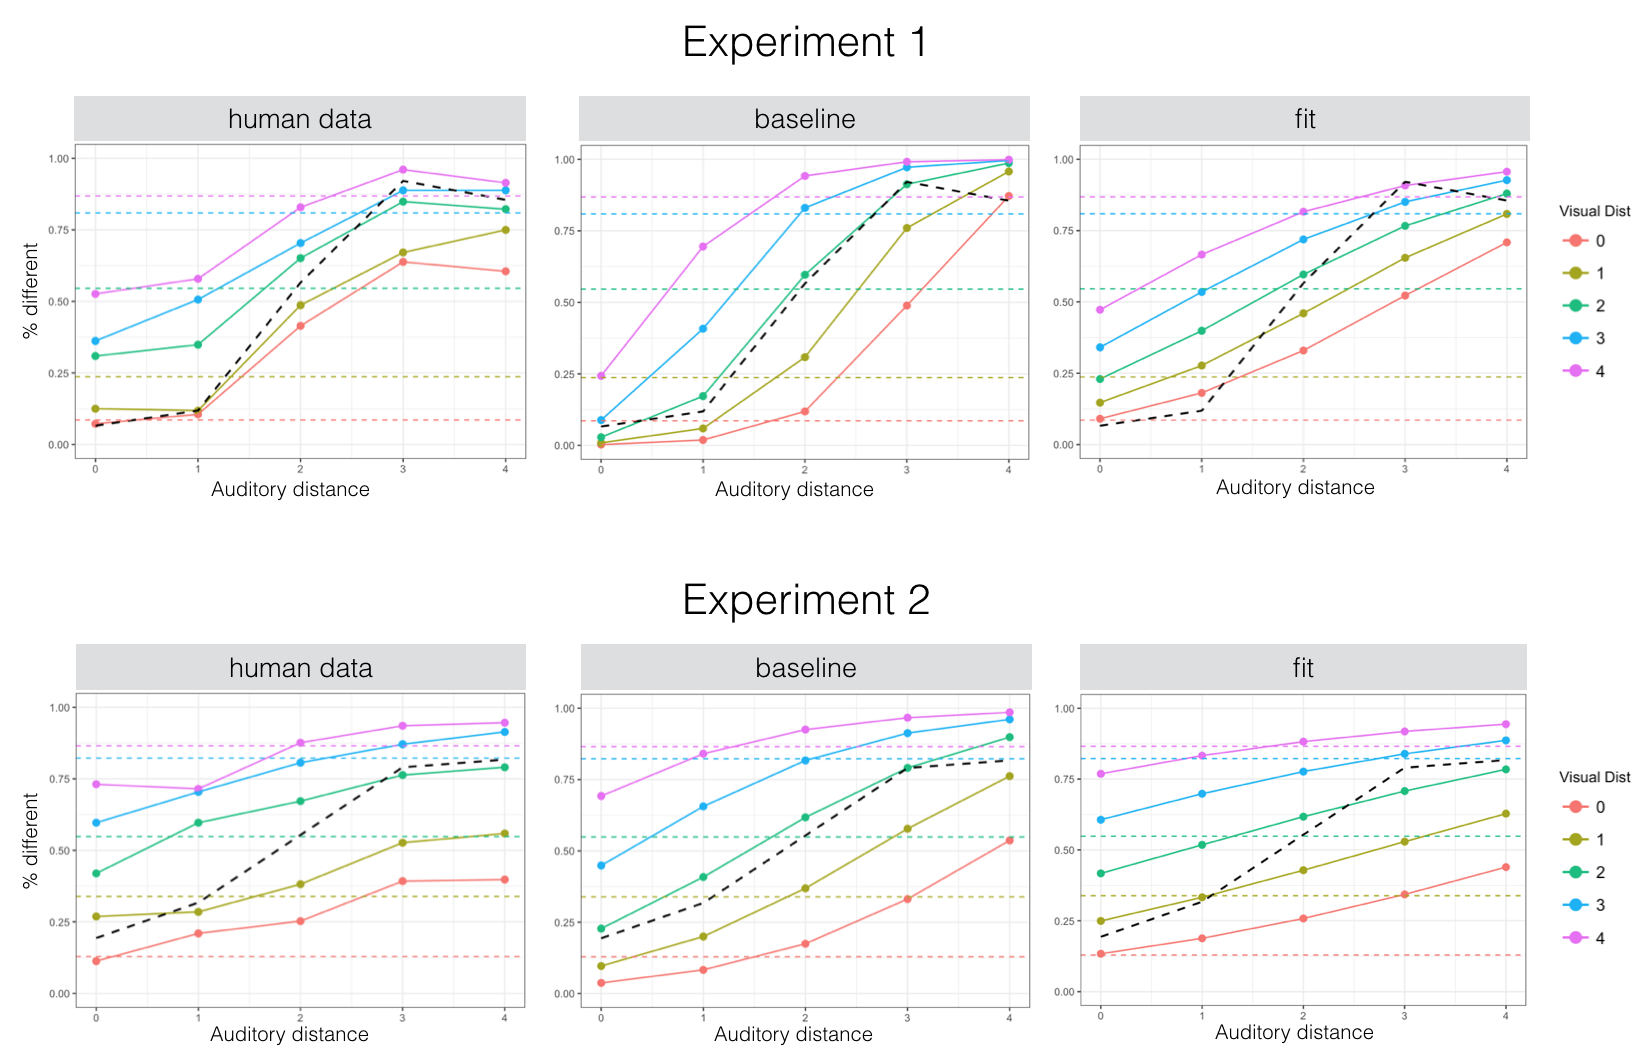
\includegraphics[width=0.83\textwidth]{Exp.png}
\caption{Proportion of `different' as a function of the auditory distance. Solid lines represent average human responses (left), predictions of the baseline (middle), and the bimodal fit (left). Dotted lines represent average human responses in the unimodal conditions. Colors represent values in the visual continuum. }
\label{fig:Exp}
\end{figure*}

\textit{Unimodal conditions:} Let's take the auditory-only case as an example, participants can be understood as choosing one of two auditory categories. For an ideal recognizer, the probability of choosing category 2 (that is, to answer `different') when presented with an audio instance $a$ is the posterior probability of this category $p(A=2|a)$. If we assume that both categories have equal variances, the posterior probability reduces to:
\begin{equation}
p(A=2 | a)=\frac{1}{1+(1+\epsilon_A)\exp(\beta_{a0}+\beta_aa)}
\end{equation}
with $\beta_a=\frac{\mu_{A1}-\mu_{A2}}{\sigma^2_{A}}$ and  $\beta_{a0}=\frac{\mu^2_{A2}-\mu^2_{A1}}{2\sigma^2_{A}}$. $\epsilon_A$ is the response bias in the auditory-only trials.

For this model (as well all other models), we fixed the values of the means to be the end-points of the corresponding continuum: $\mu_{A1}=0$ and $\mu_{A2}=4$ (and similarly $\mu_{V1}=0$, and $\mu_{V2}=4$). To determine the values of the bias and the variance, we fitted a model for each modality, collapsed across participants. For the auditory modality, we got $\epsilon_A=-0.20$ and $\sigma^2_A=2.04$. For the visual modality, we got $\epsilon_V=-0.11$ and $\sigma^2_V=3.34$.  In figure \ref{fig:unimodal} (top) we plotted responses in the unimodal conditions as well as the unimodal fits.

\textit{Bimodal condition:} we fitted a model to human responses in the bimodal condition, collapsed across participants. We got $\epsilon=-0.32$, $\sigma^2_{Ab}=5.00$ and $\sigma^2_{Vb}=7.27$.

\textit{Baseline model:} we derived the predictions of the baseline model by using the values of the variances derived from the unimodal conditions, and the response bias derived from the bimodal condition, and by plugging these values into the expression of the posterior \ref{eq:pred}.

In figure \ref{fig:Exp} (top) we plotted the participants' responses in the bimodal condition (left), as well as the prediction of the baseline (middle) and the bimodal fit (right). Correlation of human data vs. the bimodal baseline and fit are shown in figure \ref{fig:corr} (top).



\subsubsection{Discussion}
Compare human responses (figure \ref{fig:Exp}, top left) to the baseline (figure \ref{fig:Exp}, top middle). Qualitatively speaking, the participants showed many patterns of optimal behaviour (as defined by the baseline). Let's, for instance, explore how behaviour changed when participants moved from the auditory-only case (dotted black line) to the bimodal case (solid colored lines).  We see that, similar to the baseline, higher certainty in the visual modality either towards `different' (points 3 and 4 in the visual continuum), or towards `same' (points 1 and 0), generally drove responses accordingly, i.e., either towards more 'different' (as the curves moved up, compared to the auditory-only curve), or towards more `same' responses (as the curves moved down). Moreover, the amount of change was generally a function of the strength of evidence brought by the visual modality, with, for example, responses on visual point 4 being generally `higher' than responses on visual point 3. Similarly, responses on visual 0 were generally `lower' than responses on visual 1. Similar things can be said about the pattern of change from the visual-only (dotted colored horizontal lines) to the bimodal case: at each point along the auditory scale, we see that a point of a given color was generally below its corresponding horizontal line (i.e., same color) when the evidence brought by the auditory modality pointed more toward `same' (point 0 and 1), and was above its corresponding line when evidence pointed more toward `different' (point 3 and 4 along the auditory scale). These qualitative patterns were quite similar to the baseline model. Indeed, we found that the latter explained almost 90\% of the variance  ($r^2=0.89$).

Though we see a qualitative resemblance between human data and the baseline, there were quantitative differences: predictions of the baseline were either a bit too high, or a bit too low. We can see this phenomenon clearly in the shape of the correlation graph (figure \ref{fig:corr}, top left). It is as though participants were less certain about responses than expected. Formally speaking, this translated as an increase in the value of the variance associated with each modality (compare the variance values in the baseline model to the values derived from the bimodal fit).  Since the variance characterizes the reliability of a given cue, it seems as if the bimodal presentation caused reliance on both modalities to decrease.  This effect can possibly be attributed to the arbitrary nature of the form-meaning mapping. In fact, previous studies suggest that while redundant mapping improves performance (e.g., determining the frequency of a bouncing ball from visual and auditory cues), arbitrary mappings generally tends to hinder performance (see \citeA{robinson2010} for a review).


\textit{Modality preference?} we would like to know if part of the observed discrepancy between the baseline and human responses involved a systematic preference (albeit small) for a particular modality when making decisions in the bimodal condition. This preference, if real, should manifest as a deviation from the decision threshold predicted by the baseline model. The decision threshold is defined as the set of values in the audio-visual space along which the posterior (expression \ref{eq:pred}) is equal to 0.5. As illustrated in \ref{fig:space}, above this line participants are more likely to choose one word category, and below this line, they are more likely to choose the other word category. 
The decision threshold takes the following form:
\begin{equation}
v=-\frac{\sigma^2_V}{\sigma^2_A}a+v_0
\label{eq:threshold}
\end{equation}
If the slope derived from the fit is bigger than the slope of the baseline, this would suggest a general preference for the auditory modality, and a smaller slope would suggest a general preference for the visual modality. The limit cases are when there is exclusive reliance on the auditory cue (a vertical line), and where there is exclusive reliance on the visual (a horizontal line). In figure \ref{fig:pref} (top left) we plotted some decision thresholds in the audio-visual space when the intercept was kept constant. The fit to human data  (solid black line) was very close to the baseline threshold (red line). Indeed non-parametric bootstrap sampling over the data showed no proof of significant deviation from the baseline (\ref{fig:pref}, bottom left).

Finally, we found negative values in all response bias terms, which suggests a general bias toward answering `different'.  This bias is probably due to the categorical nature of the task: when two items are ambiguous but perceptually different, this could cause a slight preference for `different' over `same'. 



\subsection{experiment 2}

In experiment 1, we tested the ability of people to recognize a word category under ambiguous tokens. In particular, the tokens were clear but their category membership was uncertain. In real life situations, however, even the identity of the token can be uncertain due to various distorting factors. In order to account for this kind of uncertainty in the auditory modality, we can imagine, following \citeA{feldman2009}, that the speaker generates a target production $t$ from an auditory category
$t | A \sim N(\mu_{A}, \sigma^2_{A})$. The Listener, in a noisy condition, does not hear exactly this produced target, but the target with noise, which is assumed to be normally distributed: $a | t \sim N(t, \sigma^2_{N})$. When we integrate over $t$, we get:
\begin{equation}
a | A \sim N(\mu_{A}, \sigma^2_{A}+\sigma^2_{N})
\end{equation}
In this experiment, we explored the effect of noise on performance in our audio-visual recognition task. More precisely, we tested a case where one modality was ambiguous and noisy (auditory), and where the other modality was ambiguous but not noisy (visual). We were interested to know if participants would treat this new source of uncertainty as predicted by the optimal baseline, and whether noise in one modality would trigger some systematic preference for the non-noisy modality?   
\subsubsection{Participants}

100 participants were recruited online through Amazon Mechanical Turk. We used similar exclusion criteria as in the previous experiment. The final sample consisted of 93 participants.

\subsubsection{Stimuli}
We used the exact same visual stimuli. As for the auditory stimuli, we used the same /aba/-/ada/ continuum as in experiment 1, but we convoluted each item with Brown noise of amplitude 1 using the audio editor Audacity (2.1.2). 

\subsubsection{Procedure}
The procedure was exactly the same as in the previous experiment, except that the auditory stimuli in the test were replaced by the new noisy stimuli. The latter were not used for the target item nor during the training part. 

\subsubsection{Results}

\textit{Unimodal conditions:} we fitted a model for each modality, collapsed across participants. For the auditory modality, we got $\epsilon_A=-0.18$ and $\sigma^2_A+\sigma^2_N=4.70$. For the visual modality, we got $\epsilon_V=-0.24$ and $\sigma^2_V=3.93$.  In figure \ref{fig:unimodal} (bottom) we plotted responses in the unimodal conditions as well as the unimodal fits.

\textit{Bimodal condition:} we fitted a model to human responses in the bimodal condition, collapsed across participants. We got $\epsilon=-0.38$, $\sigma^2_{Vb}=5.21$, and  $\sigma^2_{Ab}+\sigma^2_{Nb}=9.84$. 

\textit{Baseline model:} we generated the predictions of the baseline model by using the values of the variances derived from the unimodal conditions, and the response bias derived from the bimodal condition, and by plugging these values into the expression of the posterior (expression \ref{eq:pred}).

Results are shown on  figure \ref{fig:Exp} (bottom).  Correlation of human data to the bimodal baseline and the fit are shown in figure \ref{fig:corr} (bottom). 

\subsubsection{Discussion}

\begin{figure}[h]
\centering
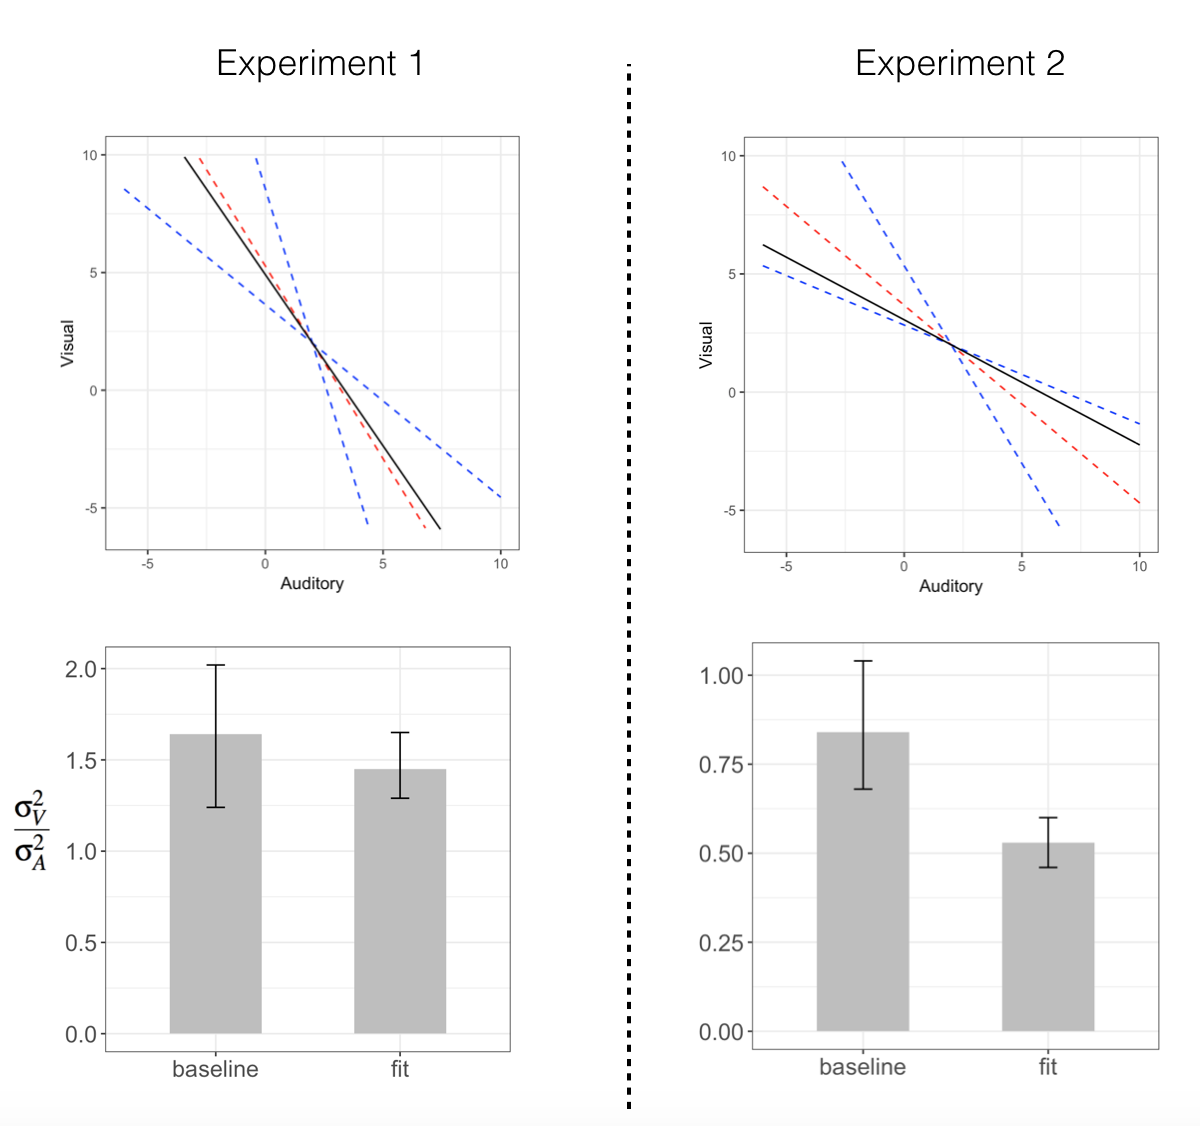
\includegraphics[width=0.4\textwidth]{preference.png}
\caption{Top: decision thresholds in the audio-visual space. Red dotted line is the prediction of the baseline. Blue dotted lines are cases where modality preference is twice as strong as the baseline. Solid line is the threshold derived from human data. Bottom: comparison of the threshold slope between the baseline and the fit to human data. Error bars are 95\% confidence intervals computed through non-parametric bootstrap sampling (10.000 samples)}
\label{fig:pref}
\end{figure}

We found, similar to experiment 1, that participants generally showed qualitative patterns similar to the baseline model. The latter explained 91\% of total variance. We also found a similar discrepancy at the quantitative level: there was a decrease in the reliability of both modalities, as could be inferred from the increase in the variance associated with the auditory modality and the visual modality in the bimodal fit. 

An interesting difference with experiment 1, however, was that participants' decision threshold suggested a preference for the visual modality (the non-noisy modality). Indeed non-parametric bootstrap sampling over the data showed there to be a significant decrease in the value of the slope. 

\section{Conclusion}


In this work, we tested word category recognition under audio-visual uncertainty. We modeled uncertainty as a probability distribution over tokens from auditory and visual continua. Our baseline model proposed a way these probability distributions can be combined in an ideal way. The model's predictions were examined in two experiments where we tested two kinds of uncertainty: in experiment 1, audio-visual tokens were clear but their category membership was ambiguous. In experiment 2, input to one modality was ambiguous, and input to the other was ambiguous as well as noisy. In both experiments, participants showed many patterns of optimal behaviour, with the model's predictions explaining 89\% and 91\% of the variance, respectively. We found, however, that a bimodal presentation caused the reliability of both modalities to decrease.
We explored whether part of the unexplained variance could involve to a systematic preference for a given modality. Our analysis showed no evidence of such modality preference in experiment 1. However, we found a preference for the non-noisy modality in experiment 2.  

This paper addressed the problem of recognizing words whose underlying phonemic and semantic categories were supposed to be familiar. An intriguing challenge is to understand how these underlying categories are acquired in the first place. Previous developmental work addressed cases when one modality was supposed to provide a stable and certain cue to the other modality \cite<e.g.,>{waxman1995, yeung09}. The present paper invites investigations on category acquisition in the more general case where there is uncertainty in both modalities.
 





\bibliographystyle{apacite}

\setlength{\bibleftmargin}{.125in}
\setlength{\bibindent}{-\bibleftmargin}

\bibliography{CogSci_Template}


\end{document}
